\newpage
\textbf{\textcolor{MidnightBlue}{4.}}
Decimos que un canal de comunicación entre dos procesos $p_i$ y $p_j$ es \code{FIFO} si los
mensajes se reciben en el mismo orden en el que se envían. Entonces, si el canal \code{NO}
es \code{FIFO}, puede ser que $p_i$ envía primero $M_1$ y después $M_2$, pero $p_j$
reciba primero $M_2$ y después $M_1$.\\

Dados dos procesos que comparten un canal $C$ que no es \code{FIFO}, da un algoritmo que
implemente un canal \code{FIFO} sobre $C$. Tu algoritmo debe tener dos secciones: una sección
{\bf send}, que recibe como entrada un mensaje $M$ a enviarse (el cuál se envía finalmente
por $C$), y una sección {\bf receive}, que recibe un mensaje $M$ de $C$ y lo entrega. De esta
forma, otro algoritmo que esté diseñado para canales \code{FIFO} puede usar tu algoritmo para
enviar y recibir mensajes. Este esquema se puede observar en la figura 2. Argumenta que tu
algoritmo es correcto. Tip: piensa en \code{timestamps} y considera que un mensaje que se
recibe de $C$ no tiene que entregarse inmediatamente.

\begin{center}
    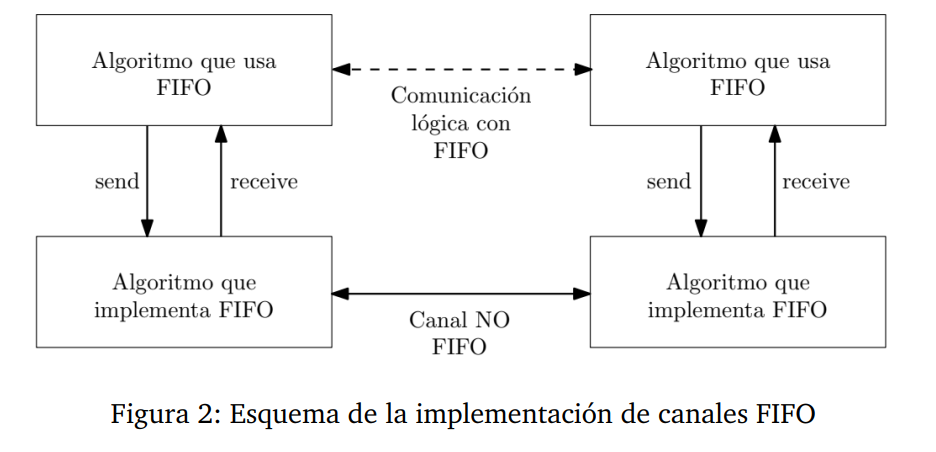
\includegraphics[scale=0.5]{Grapho1.png}
    \end{center}
